\documentclass{beamer}\usepackage[]{graphicx}\usepackage[]{color}
%% maxwidth is the original width if it is less than linewidth
%% otherwise use linewidth (to make sure the graphics do not exceed the margin)
\makeatletter
\def\maxwidth{ %
  \ifdim\Gin@nat@width>\linewidth
    \linewidth
  \else
    \Gin@nat@width
  \fi
}
\makeatother

\definecolor{fgcolor}{rgb}{0.345, 0.345, 0.345}
\newcommand{\hlnum}[1]{\textcolor[rgb]{0.686,0.059,0.569}{#1}}%
\newcommand{\hlstr}[1]{\textcolor[rgb]{0.192,0.494,0.8}{#1}}%
\newcommand{\hlcom}[1]{\textcolor[rgb]{0.678,0.584,0.686}{\textit{#1}}}%
\newcommand{\hlopt}[1]{\textcolor[rgb]{0,0,0}{#1}}%
\newcommand{\hlstd}[1]{\textcolor[rgb]{0.345,0.345,0.345}{#1}}%
\newcommand{\hlkwa}[1]{\textcolor[rgb]{0.161,0.373,0.58}{\textbf{#1}}}%
\newcommand{\hlkwb}[1]{\textcolor[rgb]{0.69,0.353,0.396}{#1}}%
\newcommand{\hlkwc}[1]{\textcolor[rgb]{0.333,0.667,0.333}{#1}}%
\newcommand{\hlkwd}[1]{\textcolor[rgb]{0.737,0.353,0.396}{\textbf{#1}}}%
\let\hlipl\hlkwb

\usepackage{framed}
\makeatletter
\newenvironment{kframe}{%
 \def\at@end@of@kframe{}%
 \ifinner\ifhmode%
  \def\at@end@of@kframe{\end{minipage}}%
  \begin{minipage}{\columnwidth}%
 \fi\fi%
 \def\FrameCommand##1{\hskip\@totalleftmargin \hskip-\fboxsep
 \colorbox{shadecolor}{##1}\hskip-\fboxsep
     % There is no \\@totalrightmargin, so:
     \hskip-\linewidth \hskip-\@totalleftmargin \hskip\columnwidth}%
 \MakeFramed {\advance\hsize-\width
   \@totalleftmargin\z@ \linewidth\hsize
   \@setminipage}}%
 {\par\unskip\endMakeFramed%
 \at@end@of@kframe}
\makeatother

\definecolor{shadecolor}{rgb}{.97, .97, .97}
\definecolor{messagecolor}{rgb}{0, 0, 0}
\definecolor{warningcolor}{rgb}{1, 0, 1}
\definecolor{errorcolor}{rgb}{1, 0, 0}
\newenvironment{knitrout}{}{} % an empty environment to be redefined in TeX

\usepackage{alltt}

%\usepackage[ngerman]{babel} % Umlaute, neue deutsche Rechtschreibung
%\usepackage[latin1]{inputenc} % Kodierung festlegen 
\usepackage{amsmath,amsfonts,amssymb} % math. Symbole und Umgebungen 
\usepackage{booktabs}
\usetheme{PaloAlto}
\IfFileExists{upquote.sty}{\usepackage{upquote}}{}
\begin{document}
%\SweaveOpts{concordance=TRUE}


\title{Introduction to R}
\author{S. Trahasch, S. Niro} 
\maketitle

\begin{frame}[fragile]
\frametitle{Goals}
\begin{itemize}
\item Know basic concepts of R
\item Be able to use essential data structures and commands
\item Create simple data visualizations
\item Be able to install and use R packages
\end{itemize}
\end{frame}

\tableofcontents

\section{Introduction}
\begin{frame}
\frametitle{Introduction (kdnuggets.com Survey 2015-2017)}
\begin{center}
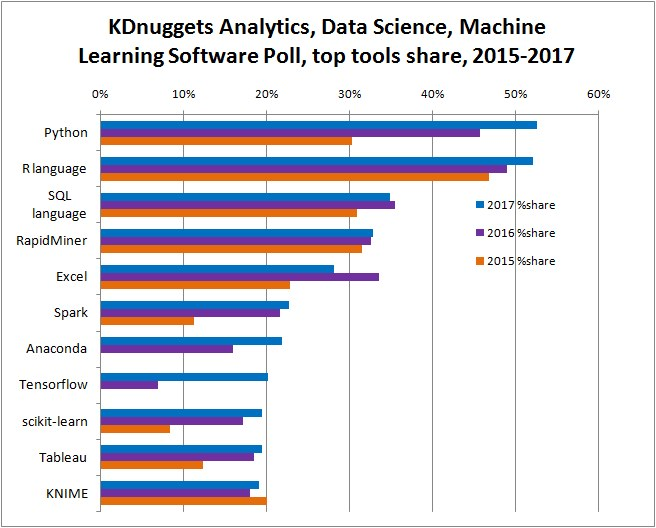
\includegraphics[scale=.35]{new_DM_polls/top-analytics-data-science-machine-learning-software-2015-2017.jpg}
\end{center}
\end{frame}

\begin{frame}
\frametitle{Introduction (kdnuggets.com Survey 2015-2017)}
\begin{center}
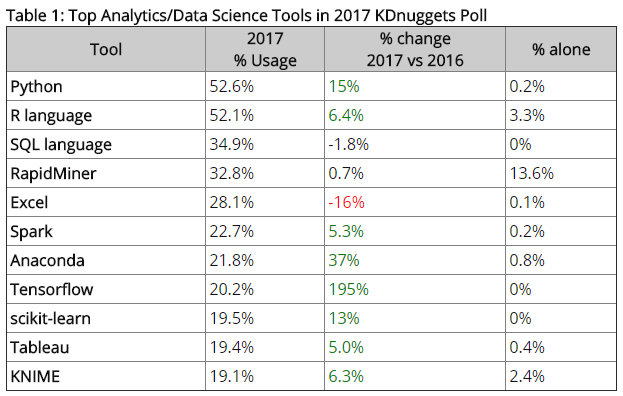
\includegraphics[scale=.5]{new_DM_polls/changes.png}
\end{center}
\end{frame}

\begin{frame}
\frametitle{Introduction}
\begin{center}
\begin{figure}
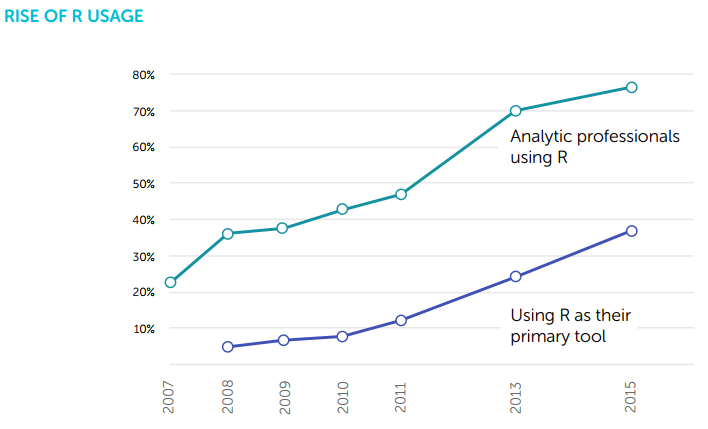
\includegraphics[scale=0.45]{new_DM_polls/rise_of_r_usage_rexeranalytics_2015.png}
\caption{Rexer Analytics Data Miner Survey 2015}
\end{figure}
\end{center}
\end{frame}

\begin{frame}
\frametitle{Introduction}
\begin{figure}
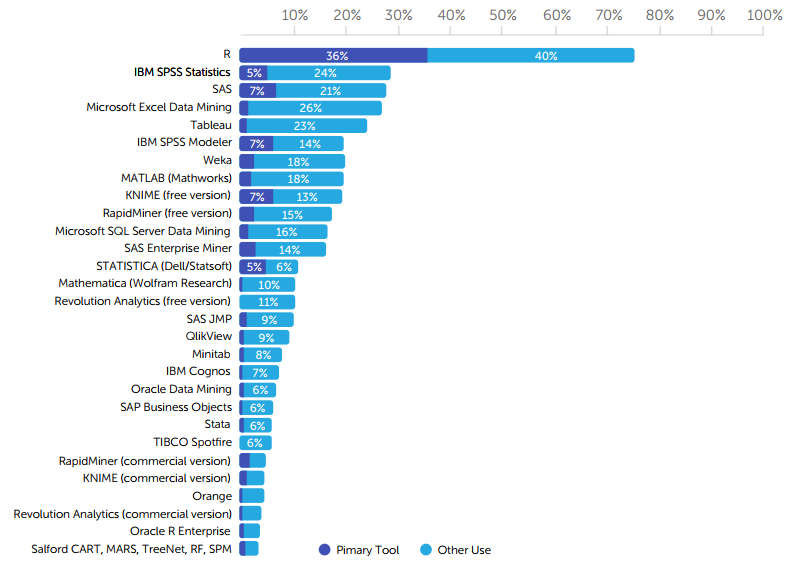
\includegraphics[scale=0.4]{new_DM_polls/primary_tool_rexeranalytics_2015.png}
\caption{Rexer Analytics Data Miner Survey 2015}
\end{figure}
\end{frame}

\section{R}

\subsection{S, S-Plus, R}

\begin{frame}
\frametitle{History: S, S-Plus, R}
\begin{itemize} 
\item Becker, R. A. und Chambers, J. M. publish \textbf{S} in 1984, a language for 
\textbf{data analysis (statistics)} and \textbf{graphics}
\item \textbf{S-PLUS} is a commercial implementation of S
\item \textbf{R} is an open source implementation of S developed in 1992 by \textbf{R}oss Ihaka and \textbf{R}obert Gentleman
\end{itemize}
\end{frame}

\subsection{Advantages of R}

\begin{frame}
\frametitle{Advantages of R}
\begin{itemize}
\item Domain specific language for data analysis and visualization
\item Open Source, no license costs (GNU GPL)
\item Huge active community
\item Available for all platforms: Windows, Linux, Solaris, ..
\item Huge number of packages ($> 10000$). New methods are often implemented and provided as (free) R-Packages
\item Faster than S-Plus
\item Bindings/Interfaces for several programming languages available (Java, Python, ... )
\item Integration of R into other data analysis software (Rapidminer, SAP HANA, SPSS, SAS, ... )
\end{itemize}
\end{frame}

\begin{frame}
\frametitle{Graphics with R - Examples (Number of R-Packages)}
\begin{figure}
\centering
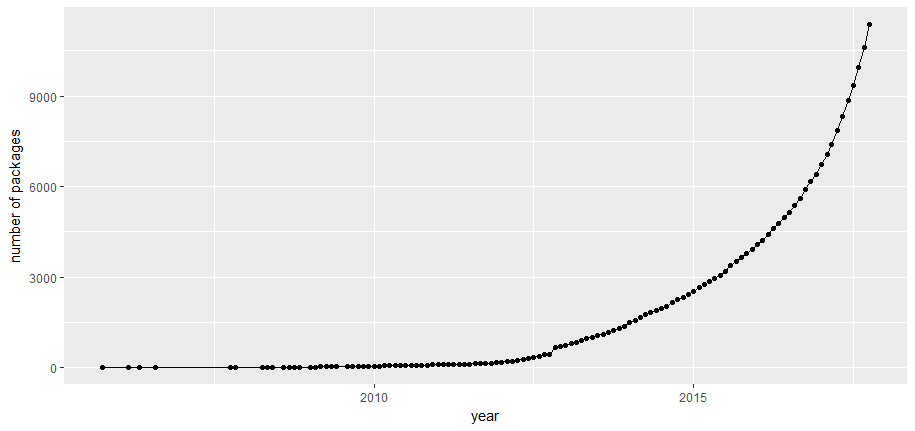
\includegraphics[scale=0.4]{new_DM_polls/rpackages_over_time.png}
\end{figure}
\end{frame}

\begin{frame}
\frametitle{Graphics with R - Examples}
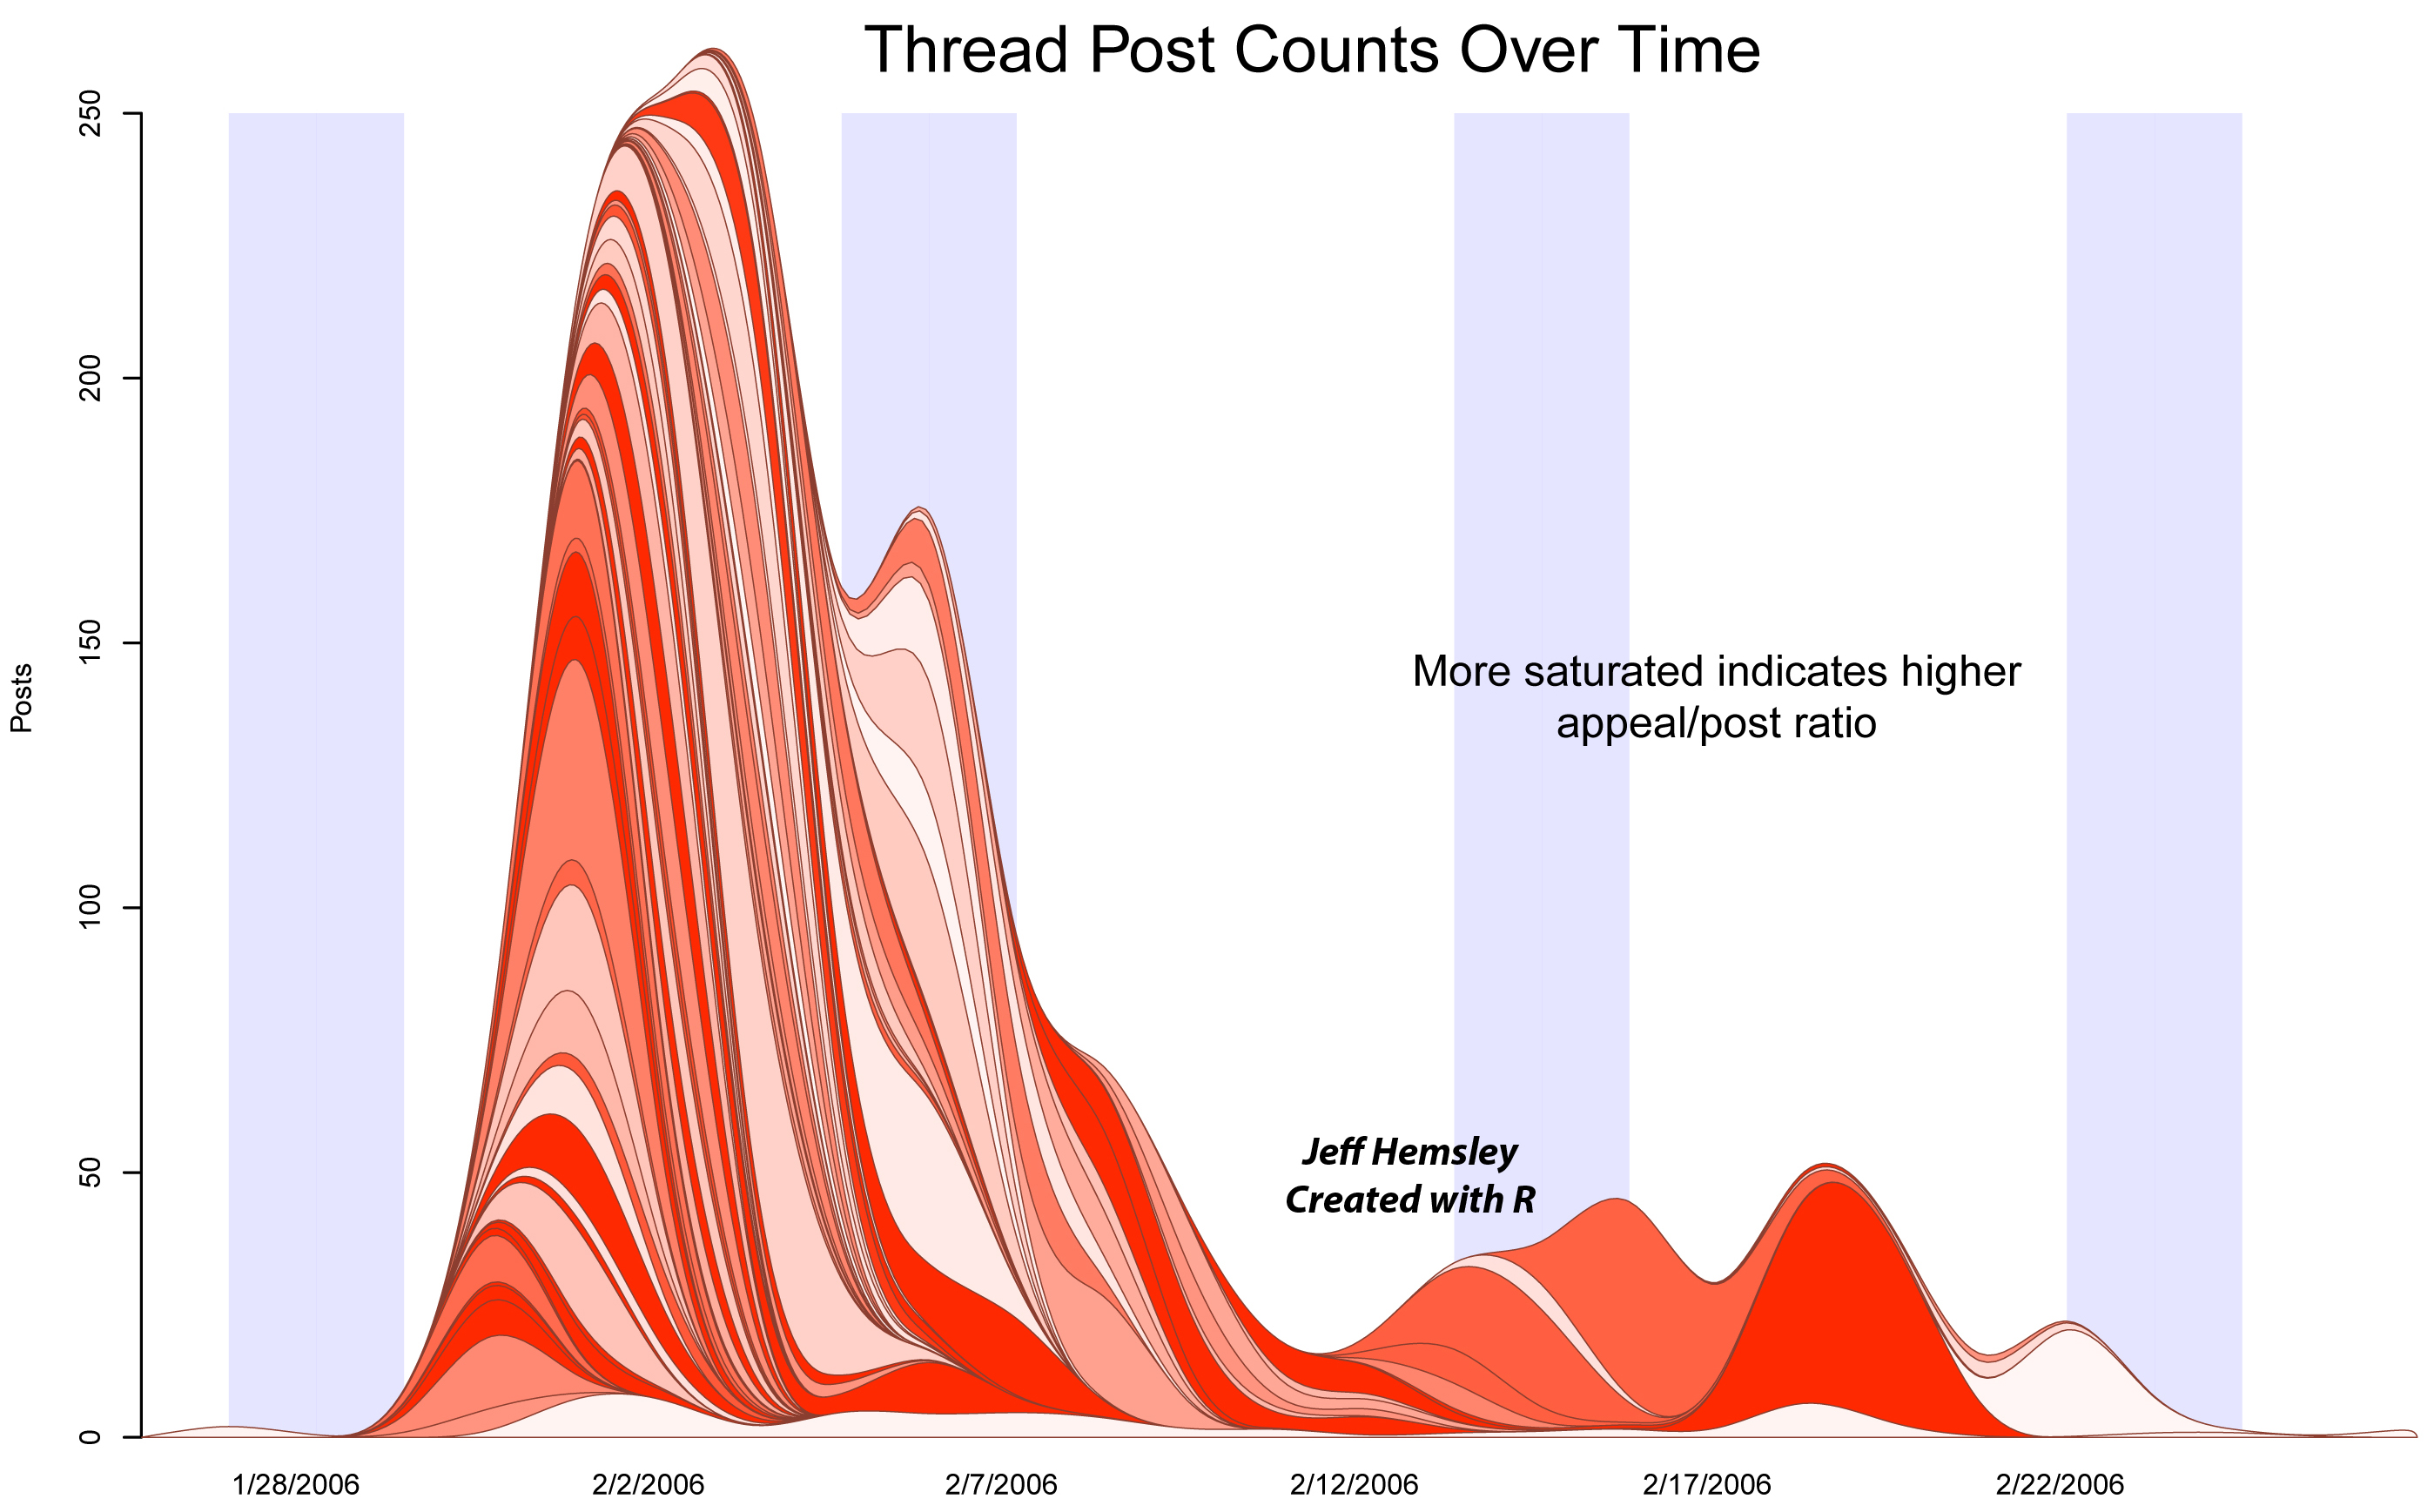
\includegraphics[scale=0.4]{pics/Jhemsley_WikiTalkPage.jpg}
\end{frame}

\begin{frame}
\frametitle{Graphics with R - Examples}
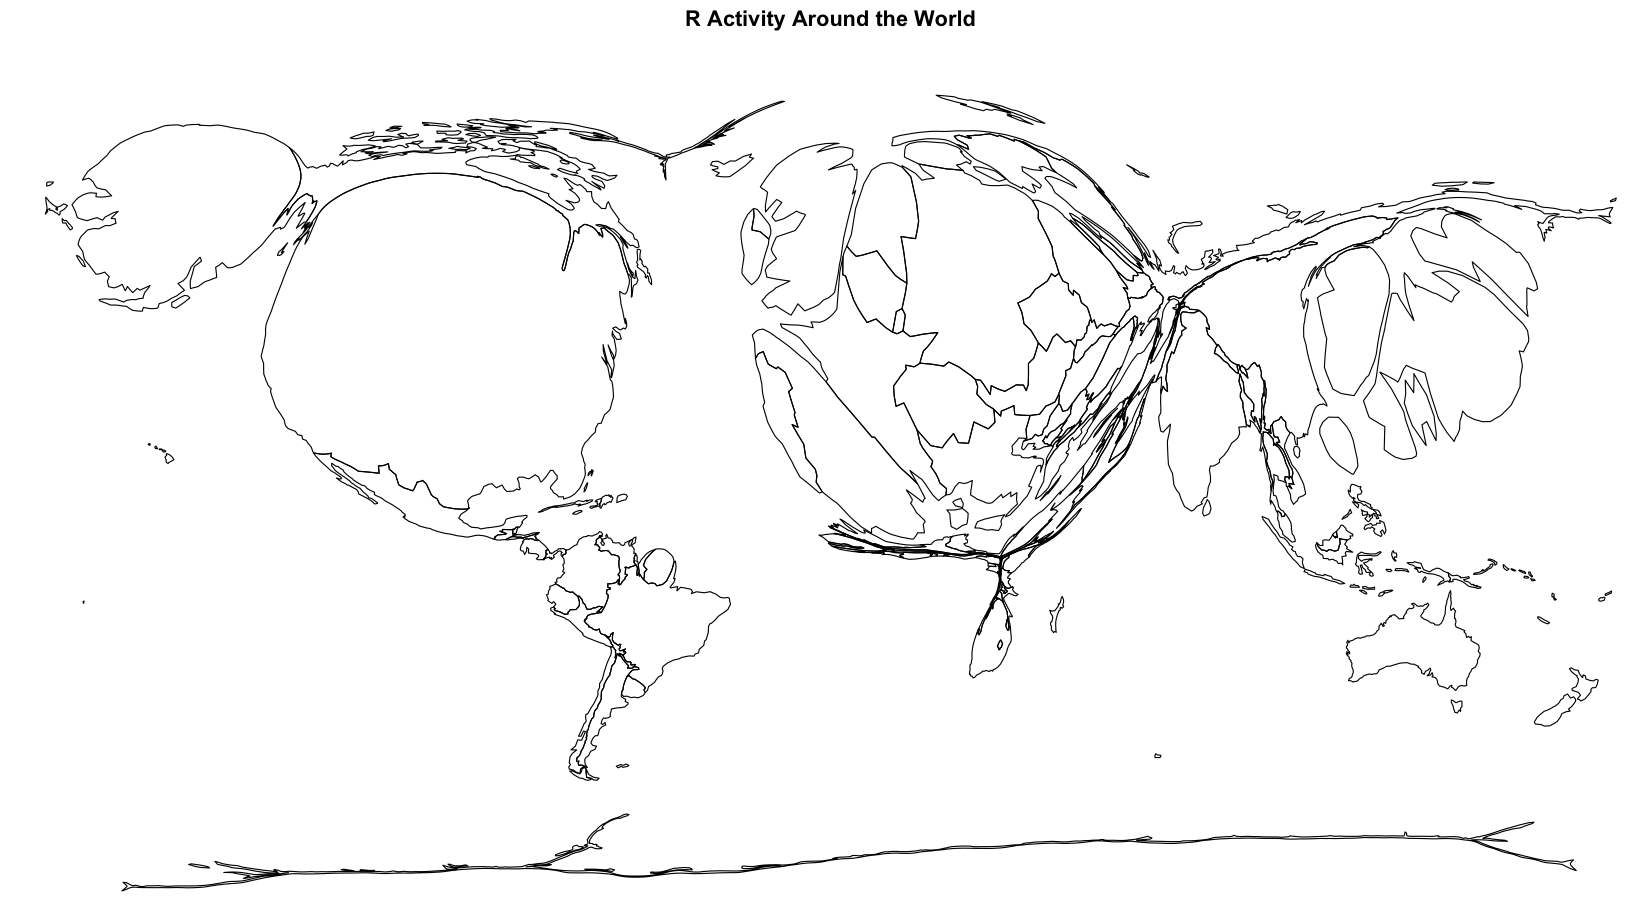
\includegraphics[scale=0.18]{pics/r_activity.png}
\end{frame}

\begin{frame}[fragile]
\frametitle{Graphics with R - Examples}
\begin{knitrout}\footnotesize
\definecolor{shadecolor}{rgb}{0.969, 0.969, 0.969}\color{fgcolor}

{\centering 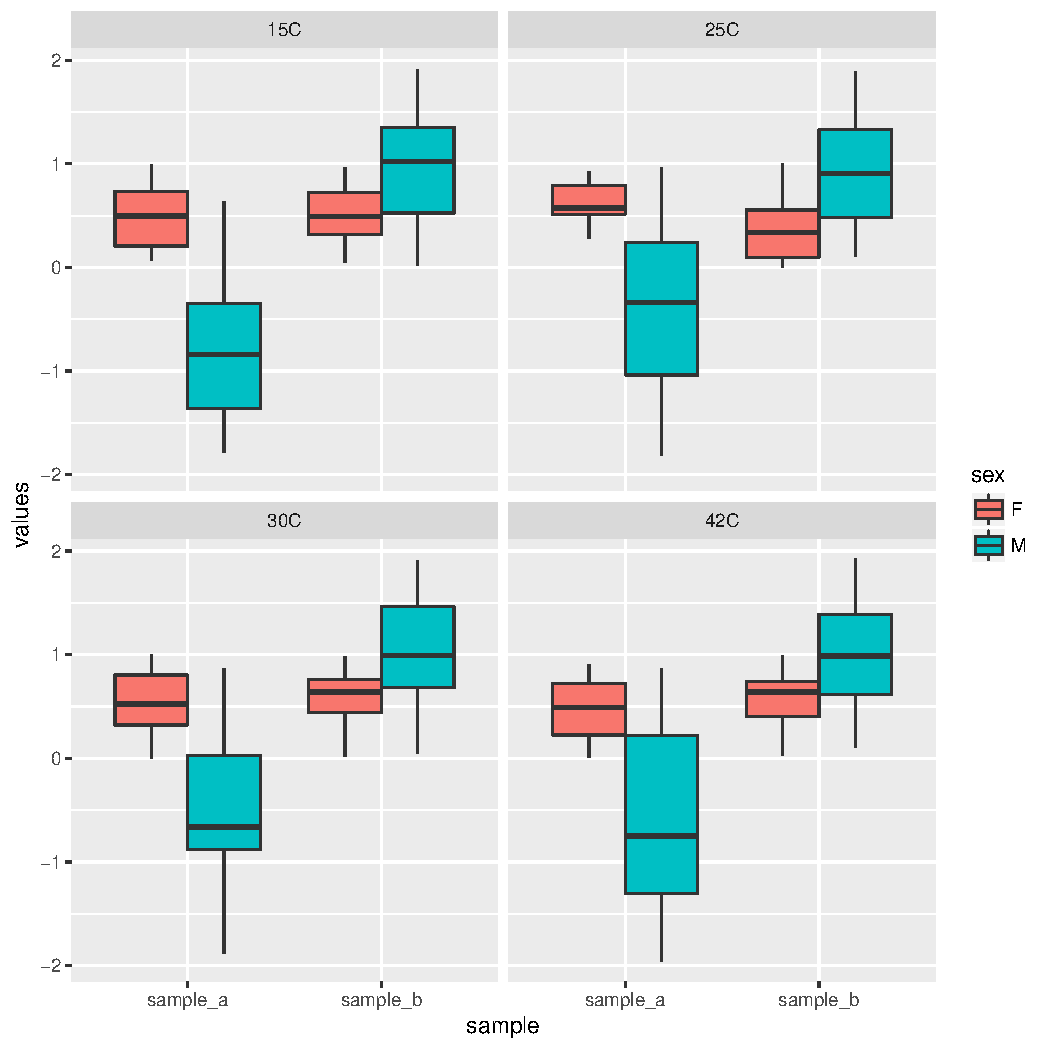
\includegraphics[width=\maxwidth]{figure/beamer-foo-1} 

}



\end{knitrout}
\end{frame}

\begin{frame}[fragile]
\frametitle{Graphics with R - Examples}
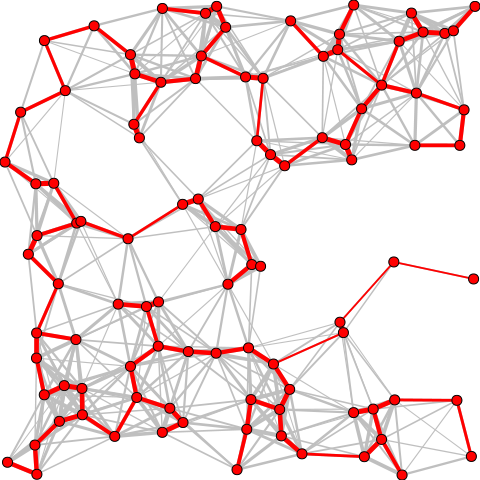
\includegraphics[scale=0.4]{pics/mst.png}
\end{frame}



\begin{frame}[fragile]
\frametitle{Graphics with R - Examples}
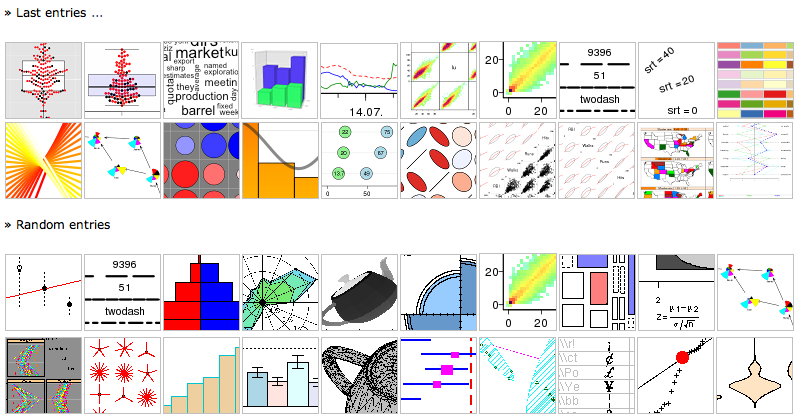
\includegraphics[scale=0.38]{pics/16a010534b1db25970b015435c323fc970c-800wi}

More: 
http://www.sr.bham.ac.uk/~ajrs/R/r-gallery.html
http://addictedtor.free.fr/graphiques/
\end{frame}

\begin{frame}[fragile]
\frametitle{Grpahics (Dilbert)}

\includegraphics[scale=0.6]{funny/I2X7z.png}
\end{frame}

\subsection{Disadvantages of R}

\begin{frame}[fragile]
\frametitle{Disadvantage of R}
\begin{itemize}
\item No graphical user interface
\item Flat learning curve compared to other data analysis software
\item Quality of the packages depends on the number of users
\item Error messages sometimes hard to interpret
\end{itemize}
\end{frame}

\section{Calculations with R}

\begin{frame}[fragile]
\frametitle{R as Calculator}
\begin{columns}[T]
    \begin{column}{.55\linewidth}
\begin{knitrout}\footnotesize
\definecolor{shadecolor}{rgb}{0.969, 0.969, 0.969}\color{fgcolor}\begin{kframe}
\begin{alltt}
\hlnum{3.5} \hlopt{+} \hlnum{1.5}
\end{alltt}
\begin{verbatim}
[1] 5
\end{verbatim}
\end{kframe}
\end{knitrout}
\begin{knitrout}\footnotesize
\definecolor{shadecolor}{rgb}{0.969, 0.969, 0.969}\color{fgcolor}\begin{kframe}
\begin{alltt}
\hlstd{x} \hlkwb{<-} \hlnum{6} \hlopt{*} \hlstd{(}\hlnum{1}\hlopt{/}\hlnum{3}\hlstd{)}  \hlcom{# Assignment}
                \hlcom{# (recommended)}
\hlstd{x}
\end{alltt}
\begin{verbatim}
[1] 2
\end{verbatim}
\end{kframe}
\end{knitrout}

\begin{knitrout}\footnotesize
\definecolor{shadecolor}{rgb}{0.969, 0.969, 0.969}\color{fgcolor}\begin{kframe}
\begin{alltt}
\hlstd{x} \hlkwb{=} \hlnum{2}\hlopt{^}\hlnum{2}       \hlcom{# Assignment}
\hlkwd{print}\hlstd{(x)}
\end{alltt}
\begin{verbatim}
[1] 4
\end{verbatim}
\end{kframe}
\end{knitrout}
    \end{column}
    \begin{column}{.45\linewidth}
     \begin{table}[cc]
     \centering
     \begin{tabular}{|c|c|} \hline
     \textbf{Operator} &  \\ \hline
      $+$ & Addition \\
      $-$ & Subtraction \\
      $*$ & Multiplication \\
      $/$ & Division \\
      \textasciicircum & Power \\ 
      $\%\%$ & Modulo \\ \hline
     \end{tabular}
    \end{table} 
    More math. functions:
    
    sin(x), sqrt(x), exp(x), ...
    
    \end{column}
  \end{columns}

\end{frame}

\section{Vectors}

\begin{frame}[fragile]
\frametitle{Vectors}
Ordered set of elements of the same type
\begin{knitrout}\footnotesize
\definecolor{shadecolor}{rgb}{0.969, 0.969, 0.969}\color{fgcolor}\begin{kframe}
\begin{alltt}
\hlstd{a} \hlkwb{<-} \hlkwd{c}\hlstd{(}\hlnum{4}\hlstd{,} \hlnum{5}\hlstd{,} \hlnum{6}\hlstd{)} \hlcom{# combine}

\hlstd{a}
\end{alltt}
\begin{verbatim}
[1] 4 5 6
\end{verbatim}
\end{kframe}
\end{knitrout}
\begin{knitrout}\footnotesize
\definecolor{shadecolor}{rgb}{0.969, 0.969, 0.969}\color{fgcolor}\begin{kframe}
\begin{alltt}
\hlkwd{length}\hlstd{(a)} \hlcom{# length of a}
\end{alltt}
\begin{verbatim}
[1] 3
\end{verbatim}
\end{kframe}
\end{knitrout}

\begin{knitrout}\footnotesize
\definecolor{shadecolor}{rgb}{0.969, 0.969, 0.969}\color{fgcolor}\begin{kframe}
\begin{alltt}
\hlstd{a[}\hlnum{2}\hlstd{]}       \hlcom{# second element of a}
\end{alltt}
\begin{verbatim}
[1] 5
\end{verbatim}
\end{kframe}
\end{knitrout}

\end{frame}

 \begin{frame}[fragile]
\frametitle{Vectors: Arithmetic}
\begin{knitrout}\footnotesize
\definecolor{shadecolor}{rgb}{0.969, 0.969, 0.969}\color{fgcolor}\begin{kframe}
\begin{alltt}
\hlstd{a} \hlkwb{<-} \hlkwd{seq}\hlstd{(}\hlkwc{from} \hlstd{=} \hlnum{1}\hlstd{,} \hlkwc{to} \hlstd{=} \hlnum{3}\hlstd{,} \hlkwc{by} \hlstd{=} \hlnum{1}\hlstd{)} \hlcom{# equals c(1,2,3)}
\hlstd{b} \hlkwb{<-} \hlnum{9}\hlopt{:}\hlnum{7} \hlcom{# equals c(9, 8, 7)}
\hlstd{a}
\end{alltt}
\begin{verbatim}
[1] 1 2 3
\end{verbatim}
\begin{alltt}
\hlstd{b}
\end{alltt}
\begin{verbatim}
[1] 9 8 7
\end{verbatim}
\end{kframe}
\end{knitrout}
\begin{columns}[T]
  \begin{column}{.5\linewidth}
  manual
\begin{knitrout}\footnotesize
\definecolor{shadecolor}{rgb}{0.969, 0.969, 0.969}\color{fgcolor}\begin{kframe}
\begin{alltt}
  \hlstd{c} \hlkwb{<-} \hlkwd{c}\hlstd{(}\hlnum{0}\hlstd{,}\hlnum{0}\hlstd{,}\hlnum{0}\hlstd{)}
  \hlkwa{for}\hlstd{(i} \hlkwa{in} \hlnum{1}\hlopt{:}\hlkwd{length}\hlstd{(a))}
  \hlstd{\{}
\hlstd{c[i]} \hlkwb{<-} \hlstd{a[i]} \hlopt{+} \hlstd{b[i]}
  \hlstd{\}}
  \hlstd{c}
\end{alltt}
\begin{verbatim}
[1] 10 10 10
\end{verbatim}
\end{kframe}
\end{knitrout}
 \end{column}
 \begin{column}{.5\linewidth}
 vectorized (recommended)
\begin{knitrout}\footnotesize
\definecolor{shadecolor}{rgb}{0.969, 0.969, 0.969}\color{fgcolor}\begin{kframe}
\begin{alltt}
\hlstd{c} \hlkwb{<-} \hlstd{a} \hlopt{+} \hlstd{b}
\hlstd{c}
\end{alltt}
\begin{verbatim}
[1] 10 10 10
\end{verbatim}
\end{kframe}
\end{knitrout}
 \end{column}


\end{columns}

\end{frame}

\def\spvec#1{\left(\vcenter{\halign{\hfil$##$\hfil\cr \spvecA#1;;}}\right)}
\def\spvecA#1;{\if;#1;\else #1\cr \expandafter \spvecA \fi}


\begin{frame}[fragile]
\frametitle{Vectors: Recycling}
\begin{knitrout}\footnotesize
\definecolor{shadecolor}{rgb}{0.969, 0.969, 0.969}\color{fgcolor}\begin{kframe}
\begin{alltt}
\hlstd{a} \hlkwb{<-} \hlnum{1}\hlopt{:}\hlnum{6}
\hlstd{a}
\end{alltt}
\begin{verbatim}
[1] 1 2 3 4 5 6
\end{verbatim}
\begin{alltt}
\hlstd{a} \hlopt{+} \hlkwd{c}\hlstd{(}\hlnum{1}\hlstd{,}\hlnum{2}\hlstd{)} \hlcom{# ???}
\end{alltt}
\begin{verbatim}
[1] 2 4 4 6 6 8
\end{verbatim}
\end{kframe}
\end{knitrout}

$\spvec{1;2;3;4;5;6} + \spvec{1;2} \longrightarrow^{recycling} \spvec{1;2;3;4;5;6} + \spvec{1;2;\color{red} 1;\color{red}2;\color{red}1;\color{red}2} = \spvec{2;4;4;6;6;8}$
\end{frame}


\begin{frame}[fragile]
\frametitle{Vectors and functions}
\begin{knitrout}\footnotesize
\definecolor{shadecolor}{rgb}{0.969, 0.969, 0.969}\color{fgcolor}\begin{kframe}
\begin{alltt}
\hlstd{a} \hlkwb{<-} \hlnum{1}\hlopt{:}\hlnum{4}
\end{alltt}
\end{kframe}
\end{knitrout}
Functions are applied to every element of the vector. The result is a new vector.
\begin{knitrout}\footnotesize
\definecolor{shadecolor}{rgb}{0.969, 0.969, 0.969}\color{fgcolor}\begin{kframe}
\begin{alltt}
\hlkwd{sqrt}\hlstd{(a)} \hlcom{# square root }
\end{alltt}
\begin{verbatim}
[1] 1.000000 1.414214 1.732051 2.000000
\end{verbatim}
\end{kframe}
\end{knitrout}

\begin{knitrout}\footnotesize
\definecolor{shadecolor}{rgb}{0.969, 0.969, 0.969}\color{fgcolor}\begin{kframe}
\begin{alltt}
\hlkwd{max}\hlstd{(a}\hlopt{^}\hlnum{2}\hlstd{)} \hlcom{# biggest element}
\end{alltt}
\begin{verbatim}
[1] 16
\end{verbatim}
\end{kframe}
\end{knitrout}

\begin{knitrout}\footnotesize
\definecolor{shadecolor}{rgb}{0.969, 0.969, 0.969}\color{fgcolor}\begin{kframe}
\begin{alltt}
\hlkwd{sum}\hlstd{(a}\hlopt{^}\hlnum{2}\hlstd{)} \hlcom{# sum of all elements}
\end{alltt}
\begin{verbatim}
[1] 30
\end{verbatim}
\end{kframe}
\end{knitrout}

\end{frame}

\begin{frame}
\frametitle{R-Studio}
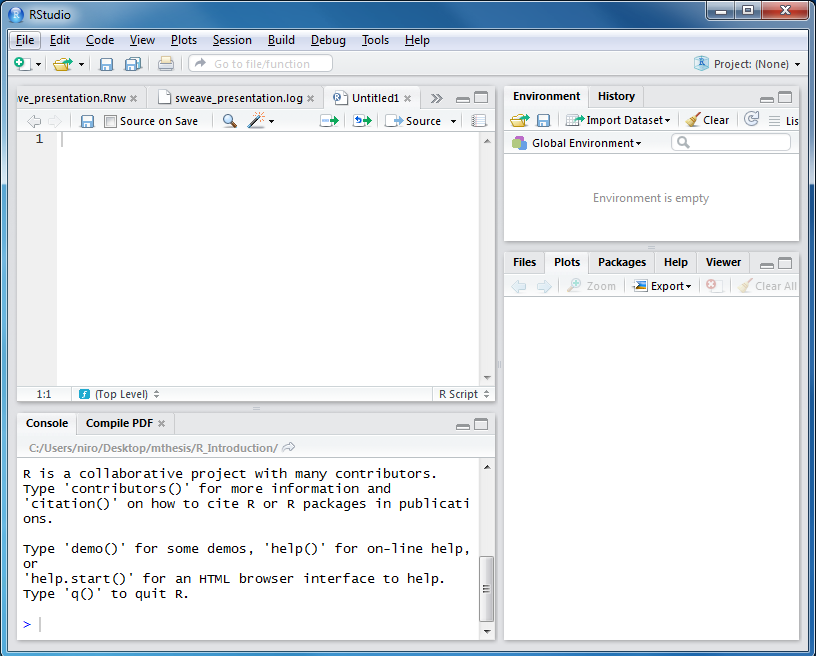
\includegraphics[scale=0.4]{pics/RStudio.png}
\end{frame}

\begin{frame}[fragile]
\frametitle{Exercise I}
\begin{itemize}
\item Create a vector $x$ of integers in the interval $[-10;10]$
\item How many elements are in $x$ (length function)?
\item Which value has the 10th and 22th element?
\item Calculate $y(x) = -x^2 + 20$
\item What is the smalles/biggest value of $y(x)$ (min/max)?
\item Plot the function $y(x)$ using plot(x, y)
\item Add the argument \begin{knitrout}\footnotesize
\definecolor{shadecolor}{rgb}{0.969, 0.969, 0.969}\color{fgcolor}\begin{kframe}
\begin{alltt}
\hlstd{type} \hlkwb{=} \hlstr{"l"}
\end{alltt}
\end{kframe}
\end{knitrout} to the plot function call. How does the plot change for 
\begin{knitrout}\footnotesize
\definecolor{shadecolor}{rgb}{0.969, 0.969, 0.969}\color{fgcolor}\begin{kframe}
\begin{alltt}
\hlstd{type} \hlkwb{=} \hlstr{"b"}
\end{alltt}
\end{kframe}
\end{knitrout}
\begin{knitrout}\footnotesize
\definecolor{shadecolor}{rgb}{0.969, 0.969, 0.969}\color{fgcolor}\begin{kframe}
\begin{alltt}
\hlstd{type} \hlkwb{=} \hlstr{"p"}
\end{alltt}
\end{kframe}
\end{knitrout}
\item Optional: Calculate $\bar{y} = \frac{1}{N} \cdot \sum_{i=1}^{N}(y_i)$
\end{itemize}
\end{frame}

\section{Exercise I}

\begin{frame}[fragile]
\frametitle{Exercise I}
\begin{columns}
  \begin{column}{0.45 \linewidth}
\begin{knitrout}\footnotesize
\definecolor{shadecolor}{rgb}{0.969, 0.969, 0.969}\color{fgcolor}\begin{kframe}
\begin{alltt}
\hlstd{x} \hlkwb{<-} \hlopt{-}\hlnum{10}\hlopt{:}\hlnum{10}
\hlkwd{length}\hlstd{(x)}
\end{alltt}
\begin{verbatim}
[1] 21
\end{verbatim}
\begin{alltt}
\hlstd{x[}\hlnum{10}\hlstd{]}
\end{alltt}
\begin{verbatim}
[1] -1
\end{verbatim}
\begin{alltt}
\hlstd{y} \hlkwb{<-} \hlopt{-}\hlstd{x}\hlopt{^}\hlnum{2} \hlopt{+} \hlnum{20}
\hlkwd{min}\hlstd{(y)}
\end{alltt}
\begin{verbatim}
[1] -80
\end{verbatim}
\begin{alltt}
\hlkwd{max}\hlstd{(y)}
\end{alltt}
\begin{verbatim}
[1] 20
\end{verbatim}
\end{kframe}
\end{knitrout}
  \end{column}
   \begin{column}{0.45 \linewidth}
\begin{knitrout}\footnotesize
\definecolor{shadecolor}{rgb}{0.969, 0.969, 0.969}\color{fgcolor}\begin{kframe}
\begin{alltt}
\hlkwd{plot}\hlstd{(x,y)}
\hlnum{1}\hlopt{/}\hlkwd{length}\hlstd{(y)} \hlopt{*} \hlkwd{sum}\hlstd{(y)}
\hlkwd{mean}\hlstd{(y)}
\end{alltt}
\begin{verbatim}
[1] -16.66667
[1] -16.66667
\end{verbatim}
\end{kframe}

{\centering 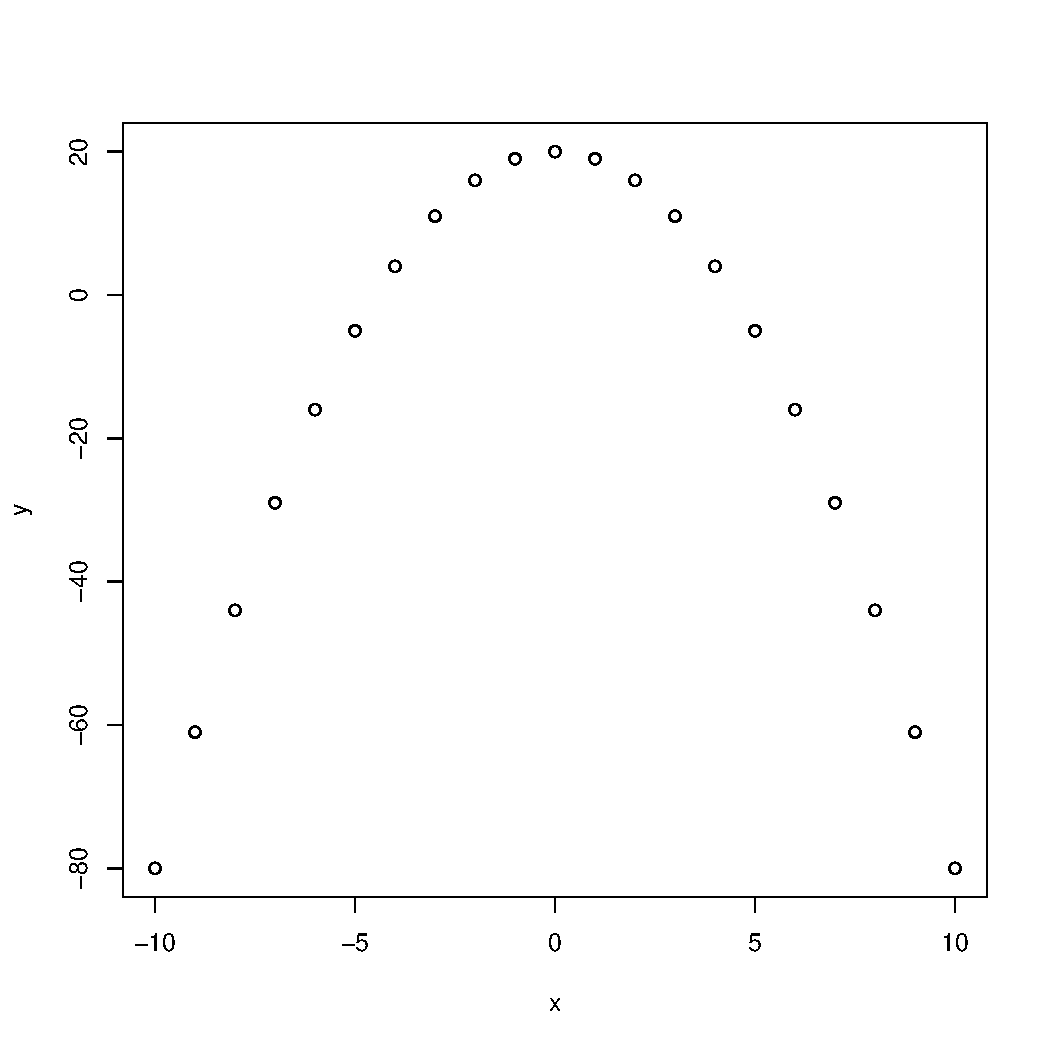
\includegraphics[width=\maxwidth]{figure/beamer-vec-uebrechts-1} 

}



\end{knitrout}
 \end{column}
 \end{columns}
\end{frame}

\section{Exercise II}

\begin{frame}[fragile]
\frametitle{Exercise II}
\begin{itemize}
\item Create $n = 100$ normal distributed random values with a mean of $10$ and a standard deviation of $1$ using the \textbf{rnorm} function (Get help using \textbf{?rnorm} or help(rnorm))
\item Calculate the mean (\textbf{mean}) and the standard deviation (\textbf{sd}) of the generated values
\item Create a boxplot (\textbf{boxplot}) and a histogram (\textbf{hist})
\item Repeat everything with $n=10000$. What changes?
\item Optional: Repeat the experiment with uniform distributed random values (\textbf{runif})
\end{itemize}
\end{frame}

\begin{frame}[fragile]
\frametitle{Exercise II (Solution)}
\begin{knitrout}\footnotesize
\definecolor{shadecolor}{rgb}{0.969, 0.969, 0.969}\color{fgcolor}\begin{kframe}
\begin{alltt}
\hlstd{x} \hlkwb{<-} \hlkwd{rnorm}\hlstd{(}\hlnum{100}\hlstd{,} \hlkwc{mean}\hlstd{=}\hlnum{10}\hlstd{,} \hlkwc{sd}\hlstd{=}\hlnum{1}\hlstd{)}
\hlkwd{mean}\hlstd{(x);} \hlkwd{sd}\hlstd{(x)}
\hlkwd{par}\hlstd{(}\hlkwc{las} \hlstd{=}\hlnum{1}\hlstd{,} \hlkwc{mar}\hlstd{=}\hlkwd{c}\hlstd{(}\hlnum{4}\hlstd{,}\hlnum{4}\hlstd{,}\hlnum{1}\hlstd{,}\hlnum{.1}\hlstd{))}
\hlkwd{boxplot}\hlstd{(x);} \hlkwd{hist}\hlstd{(x,} \hlkwc{col}\hlstd{=}\hlstr{"blue"}\hlstd{)}
\end{alltt}
\begin{verbatim}
[1] 10.05844
[1] 0.9868056
\end{verbatim}
\end{kframe}

{\centering 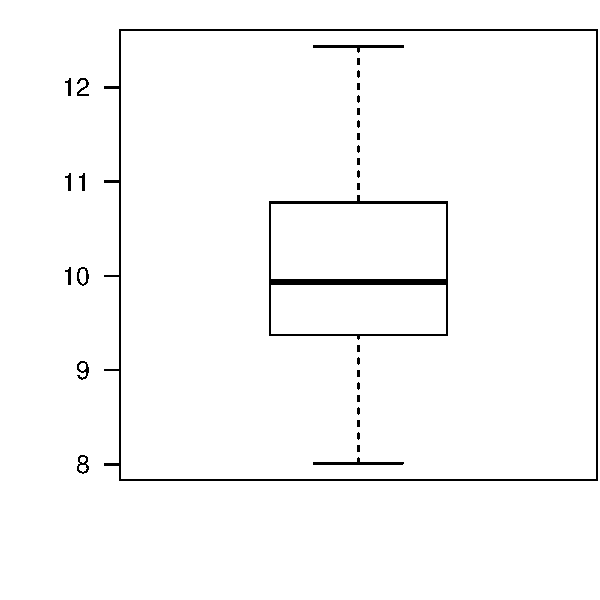
\includegraphics[width=.45\linewidth]{figure/beamer-random-first-1} 
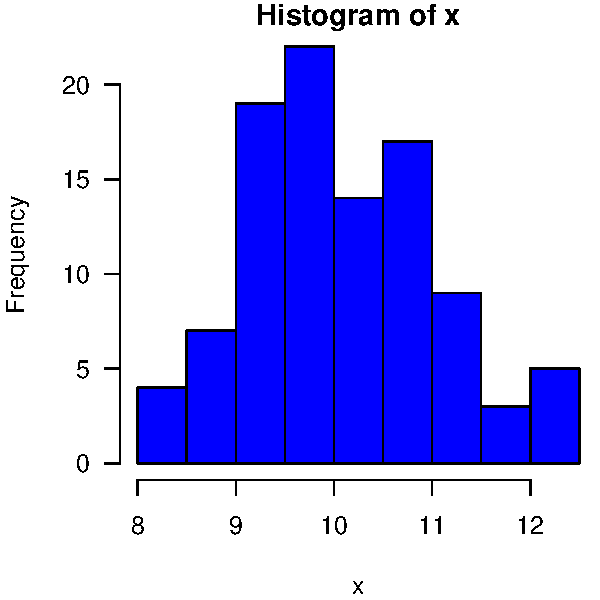
\includegraphics[width=.45\linewidth]{figure/beamer-random-first-2} 

}



\end{knitrout}
\end{frame}

\begin{frame}[fragile]
\frametitle{Exercise II (Solution)}
\begin{knitrout}\footnotesize
\definecolor{shadecolor}{rgb}{0.969, 0.969, 0.969}\color{fgcolor}\begin{kframe}
\begin{alltt}
\hlstd{x} \hlkwb{<-} \hlkwd{rnorm}\hlstd{(}\hlnum{10000}\hlstd{,} \hlkwc{mean}\hlstd{=}\hlnum{10}\hlstd{,} \hlkwc{sd}\hlstd{=}\hlnum{1}\hlstd{)}
\hlkwd{mean}\hlstd{(x);} \hlkwd{sd}\hlstd{(x)}
\hlkwd{par}\hlstd{(}\hlkwc{las} \hlstd{=}\hlnum{1}\hlstd{,} \hlkwc{mar}\hlstd{=}\hlkwd{c}\hlstd{(}\hlnum{4}\hlstd{,}\hlnum{4}\hlstd{,}\hlnum{1}\hlstd{,}\hlnum{.1}\hlstd{))}
\hlkwd{boxplot}\hlstd{(x);} \hlkwd{hist}\hlstd{(x,} \hlkwc{col}\hlstd{=}\hlstr{"blue"}\hlstd{)}
\end{alltt}
\begin{verbatim}
[1] 10.00832
[1] 1.003438
\end{verbatim}
\end{kframe}

{\centering 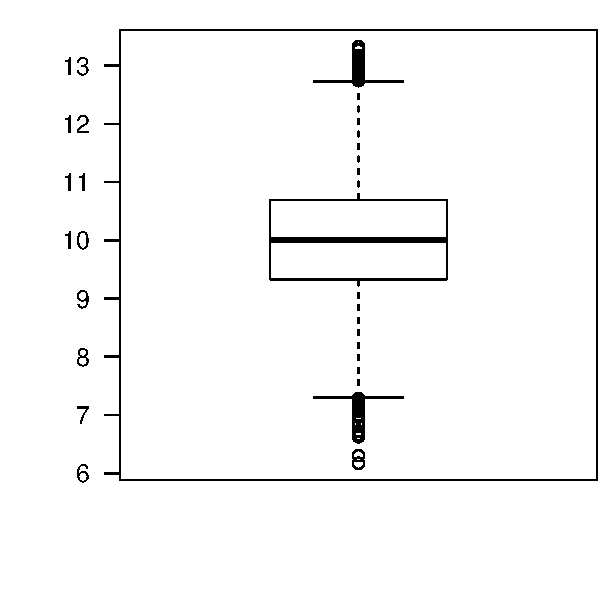
\includegraphics[width=.45\linewidth]{figure/beamer-random-second-1} 
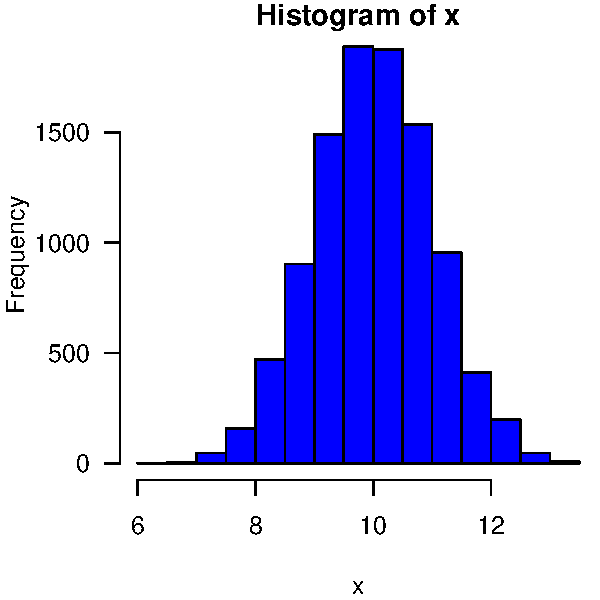
\includegraphics[width=.45\linewidth]{figure/beamer-random-second-2} 

}



\end{knitrout}
\end{frame}

\begin{frame}
\frametitle{}
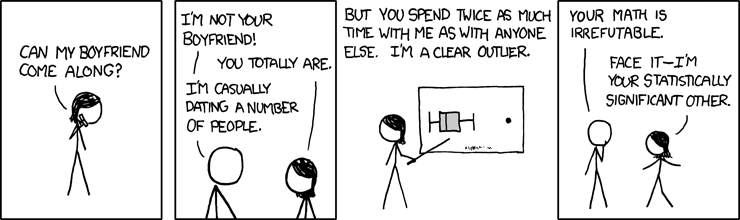
\includegraphics[scale=0.4]{funny/boyfriend.png}
\end{frame}

\begin{frame}[fragile]
\frametitle{Other types (\textit{mode})}
Logical (Boolean value)
\begin{knitrout}\footnotesize
\definecolor{shadecolor}{rgb}{0.969, 0.969, 0.969}\color{fgcolor}\begin{kframe}
\begin{alltt}
\hlstd{married} \hlkwb{<-} \hlkwd{c}\hlstd{(}\hlnum{TRUE}\hlstd{,} \hlnum{FALSE}\hlstd{, T, F, T)}
\hlkwd{print}\hlstd{(married)}
\end{alltt}
\begin{verbatim}
[1]  TRUE FALSE  TRUE FALSE  TRUE
\end{verbatim}
\end{kframe}
\end{knitrout}

Character (String)
\begin{knitrout}\footnotesize
\definecolor{shadecolor}{rgb}{0.969, 0.969, 0.969}\color{fgcolor}\begin{kframe}
\begin{alltt}
\hlstd{name} \hlkwb{<-} \hlkwd{c}\hlstd{(}\hlstr{"Max"}\hlstd{,} \hlstr{"Fritz"}\hlstd{)}
\hlkwd{print}\hlstd{(name)}
\end{alltt}
\begin{verbatim}
[1] "Max"   "Fritz"
\end{verbatim}
\end{kframe}
\end{knitrout}

Factor (Categorical values):
\begin{knitrout}\footnotesize
\definecolor{shadecolor}{rgb}{0.969, 0.969, 0.969}\color{fgcolor}\begin{kframe}
\begin{alltt}
\hlstd{sex} \hlkwb{<-} \hlkwd{factor}\hlstd{(}\hlkwd{c}\hlstd{(}\hlstr{"m"}\hlstd{,}\hlstr{"m"}\hlstd{,}\hlstr{"w"}\hlstd{,}\hlstr{"m"}\hlstd{,}\hlstr{"w"}\hlstd{,}\hlstr{"w"}\hlstd{))}
\hlkwd{print}\hlstd{(sex)}
\end{alltt}
\begin{verbatim}
[1] m m w m w w
Levels: m w
\end{verbatim}
\end{kframe}
\end{knitrout}
\end{frame}

\begin{frame}[fragile]
\frametitle{Logical and relational operators}

\begin{columns}[T]
\begin{column}{0.45 \linewidth}

\begin{knitrout}\footnotesize
\definecolor{shadecolor}{rgb}{0.969, 0.969, 0.969}\color{fgcolor}\begin{kframe}
\begin{alltt}
\hlnum{10} \hlopt{==} \hlstd{(}\hlnum{2} \hlopt{+} \hlnum{8}\hlstd{)}
\end{alltt}
\begin{verbatim}
[1] TRUE
\end{verbatim}
\begin{alltt}
\hlstd{(}\hlnum{10} \hlopt \hlnum{3} \hlopt{!=} \hlnum{0}\hlstd{)} \hlopt{&&} \hlstd{(}\hlnum{4} \hlopt{<} \hlnum{5}\hlstd{)}
\end{alltt}
\begin{verbatim}
[1] TRUE
\end{verbatim}
\begin{alltt}
\hlopt{!}\hlnum{FALSE}
\end{alltt}
\begin{verbatim}
[1] TRUE
\end{verbatim}
\end{kframe}
\end{knitrout}
\end{column}

\begin{column}{0.45 \linewidth}
\begin{table}[htbp]
  \centering
    \begin{tabular}{rrr}
    \toprule
    \textbf{Operator} & \textbf{Meaining} \\
    \midrule  
    == & Equality   \\
    !=  & Inequality \\
    $>$ &  Greater than\\
    $<=$ & Less than or equal\\
    \midrule
    Logical: & \\
    ! & NOT \\
    \&\& &  AND \\
    $||$ & OR \\

    \bottomrule
    \end{tabular}
\end{table}%
\end{column}
\end{columns}
\begin{knitrout}\footnotesize
\definecolor{shadecolor}{rgb}{0.969, 0.969, 0.969}\color{fgcolor}\begin{kframe}
\begin{alltt}
\hlkwd{c}\hlstd{(}\hlnum{5}\hlstd{,}\hlnum{8}\hlstd{,}\hlnum{10}\hlstd{)} \hlopt{>} \hlnum{5}
\end{alltt}
\begin{verbatim}
[1] FALSE  TRUE  TRUE
\end{verbatim}
\end{kframe}
\end{knitrout}
\end{frame}

\begin{frame}[fragile]
\frametitle{Conditional Execution}
\begin{knitrout}\footnotesize
\definecolor{shadecolor}{rgb}{0.969, 0.969, 0.969}\color{fgcolor}\begin{kframe}
\begin{alltt}
\hlkwa{if}\hlstd{(}\hlnum{2}\hlopt{+}\hlnum{2}\hlopt{==}\hlnum{5}\hlstd{)}
\hlstd{\{}
  \hlkwd{print}\hlstd{(}\hlstr{"2+2 equals 5"}\hlstd{)}
\hlstd{\}}\hlkwa{else}
\hlstd{\{}
  \hlkwd{print}\hlstd{(}\hlstr{"2+2 not equals 5"}\hlstd{)}
\hlstd{\}}
\end{alltt}
\begin{verbatim}
[1] "2+2 not equals 5"
\end{verbatim}
\end{kframe}
\end{knitrout}

short:
\begin{knitrout}\footnotesize
\definecolor{shadecolor}{rgb}{0.969, 0.969, 0.969}\color{fgcolor}\begin{kframe}
\begin{alltt}
\hlkwd{ifelse}\hlstd{(}\hlnum{2}\hlopt{+}\hlnum{2}\hlopt{==}\hlnum{5}\hlstd{,} \hlstr{"equal"}\hlstd{,} \hlstr{"not equal"}\hlstd{)}
\end{alltt}
\begin{verbatim}
[1] "not equal"
\end{verbatim}
\begin{alltt}
\hlkwd{ifelse}\hlstd{(}\hlnum{1}\hlopt{:}\hlnum{10}\hlopt{==}\hlnum{5}\hlstd{,} \hlstr{"equal"}\hlstd{,} \hlstr{"not equal"}\hlstd{)} \hlcom{# vectorized}
\end{alltt}
\begin{verbatim}
 [1] "not equal" "not equal" "not equal" "not equal"
 [5] "equal"     "not equal" "not equal" "not equal"
 [9] "not equal" "not equal"
\end{verbatim}
\end{kframe}
\end{knitrout}
\end{frame}

\begin{frame}[fragile]
\frametitle{Conditional selection}
\begin{knitrout}\footnotesize
\definecolor{shadecolor}{rgb}{0.969, 0.969, 0.969}\color{fgcolor}\begin{kframe}
\begin{alltt}
\hlstd{a} \hlkwb{<-} \hlkwd{c}\hlstd{(}\hlnum{2}\hlstd{,}\hlnum{4}\hlstd{,}\hlnum{6}\hlstd{,}\hlnum{8}\hlstd{,}\hlnum{10}\hlstd{)}
\end{alltt}
\end{kframe}
\end{knitrout}
\begin{knitrout}\footnotesize
\definecolor{shadecolor}{rgb}{0.969, 0.969, 0.969}\color{fgcolor}\begin{kframe}
\begin{alltt}
\hlstd{a[}\hlnum{1}\hlopt{:}\hlnum{3}\hlstd{]}  \hlcom{# Index based selection }
\end{alltt}
\begin{verbatim}
[1] 2 4 6
\end{verbatim}
\end{kframe}
\end{knitrout}
\begin{knitrout}\footnotesize
\definecolor{shadecolor}{rgb}{0.969, 0.969, 0.969}\color{fgcolor}\begin{kframe}
\begin{alltt}
\hlstd{a[}\hlkwd{c}\hlstd{(T,T,T,F,F)]} \hlcom{# Conditional selection}
\end{alltt}
\begin{verbatim}
[1] 2 4 6
\end{verbatim}
\end{kframe}
\end{knitrout}
\begin{knitrout}\footnotesize
\definecolor{shadecolor}{rgb}{0.969, 0.969, 0.969}\color{fgcolor}\begin{kframe}
\begin{alltt}
\hlstd{a[a} \hlopt{<} \hlnum{7}\hlstd{]} \hlcom{# Conditional selection}
\end{alltt}
\begin{verbatim}
[1] 2 4 6
\end{verbatim}
\end{kframe}
\end{knitrout}
\end{frame}

% DATA FRAMES
\section{Data Frame}

\begin{frame}[fragile]
\frametitle{Data Frame}
\begin{itemize}
\item List of vectors of the same length (columns) that are named
\item Important data structure
\item Example
% Table generated by Excel2LaTeX from sheet 'teilnehmer'
\begin{table}[htbp]
  \centering
    \begin{tabular}{rrr}
    \toprule
    \textbf{Name} & \textbf{Division} & \textbf{Shoesize} \\
    \midrule
    Dennis & APC   & 42 \\
    Ralf  & SIB   & 43 \\
    Stefan & IS    & 42 \\
    Susanne & APC   & 39 \\
    Swen  & SIB   & 42 \\
    Werner & SIB   & 43 \\
    \bottomrule
    \end{tabular}
    \caption{Participants as CSV-File}
\end{table}%
\item Two Indices: df[ \color{blue}  Row(s) \color{black}, \color{red} Column(s) \color{black}] 
\end{itemize}
\end{frame}

\begin{frame}[fragile]
\frametitle{Data Frame}
\begin{knitrout}\footnotesize
\definecolor{shadecolor}{rgb}{0.969, 0.969, 0.969}\color{fgcolor}\begin{kframe}
\begin{alltt}
\hlstd{df} \hlkwb{<-} \hlkwd{read.csv}\hlstd{(}\hlstr{"participants.csv"}\hlstd{,} \hlkwc{sep}\hlstd{=}\hlstr{";"}\hlstd{)}
\hlstd{df}
\end{alltt}
\begin{verbatim}
     Name Gruppe Shoesize
1  Dennis    APC       42
2    Ralf    SIB       43
3  Stefan     IS       42
4 Susanne    APC       39
5    Swen    SIB       42
6  Werner    SIB       43
\end{verbatim}
\begin{alltt}
\hlkwd{names}\hlstd{(df)}  \hlcom{# Column names}
\end{alltt}
\begin{verbatim}
[1] "Name"     "Gruppe"   "Shoesize"
\end{verbatim}
\begin{alltt}
\hlkwd{dim}\hlstd{(df)}    \hlcom{# Dimensions (rows, columns)}
\end{alltt}
\begin{verbatim}
[1] 6 3
\end{verbatim}
\end{kframe}
\end{knitrout}
\end{frame}

\begin{frame}[fragile]
\frametitle{Data Frame: Access the contents}
\begin{knitrout}\footnotesize
\definecolor{shadecolor}{rgb}{0.969, 0.969, 0.969}\color{fgcolor}\begin{kframe}
\begin{alltt}
\hlstd{df[}\hlnum{1}\hlstd{, ]} \hlcom{# first row, all columns}
\end{alltt}
\begin{verbatim}
    Name Gruppe Shoesize
1 Dennis    APC       42
\end{verbatim}
\end{kframe}
\end{knitrout}
\begin{knitrout}\footnotesize
\definecolor{shadecolor}{rgb}{0.969, 0.969, 0.969}\color{fgcolor}\begin{kframe}
\begin{alltt}
\hlstd{df[}\hlnum{1}\hlstd{,}\hlnum{3}\hlstd{]} \hlcom{# first row, third column}
\end{alltt}
\begin{verbatim}
[1] 42
\end{verbatim}
\end{kframe}
\end{knitrout}
\begin{knitrout}\footnotesize
\definecolor{shadecolor}{rgb}{0.969, 0.969, 0.969}\color{fgcolor}\begin{kframe}
\begin{alltt}
\hlstd{df[,}\hlnum{2}\hlstd{]} \hlcom{# all rows, second column}
\end{alltt}
\begin{verbatim}
[1] APC SIB IS  APC SIB SIB
Levels: APC IS SIB
\end{verbatim}
\end{kframe}
\end{knitrout}
\begin{knitrout}\footnotesize
\definecolor{shadecolor}{rgb}{0.969, 0.969, 0.969}\color{fgcolor}\begin{kframe}
\begin{alltt}
\hlstd{df[,}\hlstr{"Shoesize"}\hlstd{]} \hlcom{# Column by name I}
\end{alltt}
\begin{verbatim}
[1] 42 43 42 39 42 43
\end{verbatim}
\end{kframe}
\end{knitrout}

\end{frame}

\begin{frame}[fragile]
\frametitle{Data Frame: Access the contents II}
\begin{knitrout}\footnotesize
\definecolor{shadecolor}{rgb}{0.969, 0.969, 0.969}\color{fgcolor}\begin{kframe}
\begin{alltt}
\hlstd{df}\hlopt{$}\hlstd{Name} \hlcom{# Column by name II}
\end{alltt}
\begin{verbatim}
[1] Dennis  Ralf    Stefan  Susanne Swen    Werner 
Levels: Dennis Ralf Stefan Susanne Swen Werner
\end{verbatim}
\begin{alltt}
\hlstd{df[df}\hlopt{$}\hlstd{Shoesize} \hlopt{<} \hlnum{41}\hlstd{,]}
\end{alltt}
\begin{verbatim}
     Name Gruppe Shoesize
4 Susanne    APC       39
\end{verbatim}
\begin{alltt}
\hlstd{df[df}\hlopt{$}\hlstd{Group} \hlopt{==} \hlstr{"APC"}\hlstd{,} \hlstr{"Name"}\hlstd{]}
\end{alltt}
\begin{verbatim}
factor(0)
Levels: Dennis Ralf Stefan Susanne Swen Werner
\end{verbatim}
\end{kframe}
\end{knitrout}
\end{frame}

\begin{frame}[fragile]
\begin{knitrout}\footnotesize
\definecolor{shadecolor}{rgb}{0.969, 0.969, 0.969}\color{fgcolor}\begin{kframe}
\begin{alltt}
\hlkwd{str}\hlstd{(df)}
\end{alltt}
\begin{verbatim}
'data.frame':	6 obs. of  3 variables:
 $ Name    : Factor w/ 6 levels "Dennis","Ralf",..: 1 2 3 4 5 6
 $ Gruppe  : Factor w/ 3 levels "APC","IS","SIB": 1 3 2 1 3 3
 $ Shoesize: int  42 43 42 39 42 43
\end{verbatim}
\end{kframe}
\end{knitrout}
\begin{knitrout}\footnotesize
\definecolor{shadecolor}{rgb}{0.969, 0.969, 0.969}\color{fgcolor}\begin{kframe}
\begin{alltt}
\hlkwd{summary}\hlstd{(df)}
\end{alltt}
\begin{verbatim}
      Name   Gruppe     Shoesize    
 Dennis :1   APC:2   Min.   :39.00  
 Ralf   :1   IS :1   1st Qu.:42.00  
 Stefan :1   SIB:3   Median :42.00  
 Susanne:1           Mean   :41.83  
 Swen   :1           3rd Qu.:42.75  
 Werner :1           Max.   :43.00  
\end{verbatim}
\end{kframe}
\end{knitrout}
\end{frame}

% �bung 3
\section{Exercise III (Part 1)}

\begin{frame}[fragile]
\begin{itemize}
\frametitle{Exercise III (Part 1): Packages and Data Frames}
\item Install the two packages \textbf{rpart} and \textbf{rpart.plot}
(\textit{Tools/Install Packages ...} in RStudio or via Console with \textit{install.packages("PACKAGE\_NAME")})
\item Load both Packages with \textit{library(PACKAGE\_NAME)}
\item Load the example data set \textbf{ptitanic} with $data(ptitanic)$
\item Use the functions \textbf{summary} and \textbf{str} on the ptitanic data frame 
\item Create a scatterplot \textbf{plot} (Color the data points with the argument
\begin{knitrout}\footnotesize
\definecolor{shadecolor}{rgb}{0.969, 0.969, 0.969}\color{fgcolor}\begin{kframe}
\begin{alltt}
\hlstd{col} \hlkwb{=} \hlkwd{ifelse}\hlstd{(ptitanic}\hlopt{$}\hlstd{survived}\hlopt{==}\hlstr{" survived"}\hlstd{,} \hlstr{"green"}\hlstd{,} \hlstr{"red"}\hlstd{)}
\end{alltt}
\end{kframe}
\end{knitrout}
\end{itemize}
\end{frame}

\begin{frame}[fragile]
\frametitle{Exercise III (Part 1 Solution)}
\begin{knitrout}\footnotesize
\definecolor{shadecolor}{rgb}{0.969, 0.969, 0.969}\color{fgcolor}\begin{kframe}
\begin{alltt}
\hlkwd{library}\hlstd{(rpart);}\hlkwd{library}\hlstd{(rpart.plot);}\hlkwd{data}\hlstd{(ptitanic);} \hlkwd{options}\hlstd{(}\hlkwc{width}\hlstd{=}\hlnum{60}\hlstd{)}
\hlkwd{str}\hlstd{(ptitanic)}
\end{alltt}
\begin{verbatim}
'data.frame':	1309 obs. of  6 variables:
 $ pclass  : Factor w/ 3 levels "1st","2nd","3rd": 1 1 1 1 1 1 1 1 1 1 ...
 $ survived: Factor w/ 2 levels "died","survived": 2 2 1 1 1 2 2 1 2 1 ...
 $ sex     : Factor w/ 2 levels "female","male": 1 2 1 2 1 2 1 2 1 2 ...
 $ age     :Class 'labelled'  atomic [1:1309] 29 0.917 2 30 25 ...
  .. ..- attr(*, "units")= chr "Year"
  .. ..- attr(*, "label")= chr "Age"
 $ sibsp   :Class 'labelled'  atomic [1:1309] 0 1 1 1 1 0 1 0 2 0 ...
  .. ..- attr(*, "label")= chr "Number of Siblings/Spouses Aboard"
 $ parch   :Class 'labelled'  atomic [1:1309] 0 2 2 2 2 0 0 0 0 0 ...
  .. ..- attr(*, "label")= chr "Number of Parents/Children Aboard"
\end{verbatim}
\end{kframe}
\end{knitrout}
\end{frame}

\begin{frame}[fragile]
\frametitle{Exercise III (Part 1 Solution)}
\begin{knitrout}\footnotesize
\definecolor{shadecolor}{rgb}{0.969, 0.969, 0.969}\color{fgcolor}\begin{kframe}
\begin{alltt}
\hlkwd{summary}\hlstd{(ptitanic)}
\end{alltt}
\begin{verbatim}
 pclass        survived       sex           age         
 1st:323   died    :809   female:466   Min.   : 0.1667  
 2nd:277   survived:500   male  :843   1st Qu.:21.0000  
 3rd:709                               Median :28.0000  
                                       Mean   :29.8811  
                                       3rd Qu.:39.0000  
                                       Max.   :80.0000  
                                       NA's   :263      
     sibsp            parch      
 Min.   :0.0000   Min.   :0.000  
 1st Qu.:0.0000   1st Qu.:0.000  
 Median :0.0000   Median :0.000  
 Mean   :0.4989   Mean   :0.385  
 3rd Qu.:1.0000   3rd Qu.:0.000  
 Max.   :8.0000   Max.   :9.000  
                                 
\end{verbatim}
\end{kframe}
\end{knitrout}
\end{frame}

\begin{frame}[fragile]
\frametitle{Exercise III (Part 1 Solution)}
\begin{knitrout}\footnotesize
\definecolor{shadecolor}{rgb}{0.969, 0.969, 0.969}\color{fgcolor}\begin{kframe}
\begin{alltt}
\hlkwd{plot}\hlstd{(ptitanic,} \hlkwc{col} \hlstd{=} \hlkwd{ifelse}\hlstd{(ptitanic}\hlopt{$}\hlstd{survived} \hlopt{==} \hlstr{"survived"}\hlstd{,}
    \hlstr{"green"}\hlstd{,} \hlstr{"red"}\hlstd{))}
\end{alltt}
\end{kframe}

{\centering 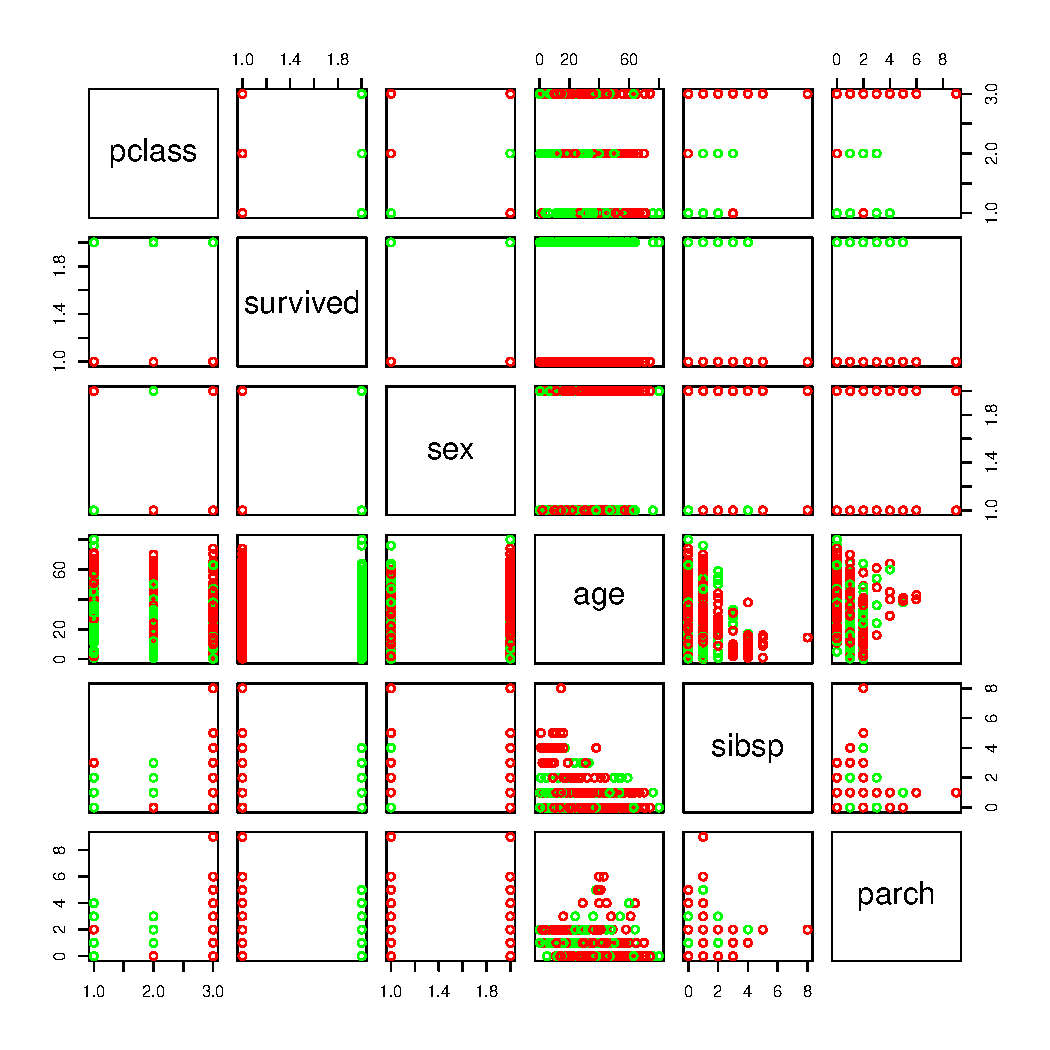
\includegraphics[width=\maxwidth,height=0.5\linewidth]{figure/beamer-titanic-third} 

}



\end{knitrout}
\begin{minipage}[t]{0.48\linewidth}
\end{minipage}%
\end{frame}

\section{Excursion}

\begin{frame}
\frametitle{Excursion: Data-Mining I}
\begin{itemize}
\item Goal: Discover unknown relationships in the data using algorithms
\item Here: Find out what properties (attributes) determined whether a passenger survived the catastrophe or not

\begin{table}[htbp]
  \centering
    \begin{tabular}{rrr|r}
    \toprule
    \textbf{$x_1$} &  ... & \textbf{$x_i$} & $y$ \\
    \midrule
    1&..&1& survived\\
    1&..&1& died\\
    2&..&1& survived\\
    \midrule
    1&..&1& ?\\
    1&..&1& ?\\
    2&..&5& ?\\    
    \bottomrule
    \end{tabular}
    %\caption{Data are provided in tabular form}
\end{table}%

\end{itemize}
\end{frame}


\begin{frame}
\frametitle{Excursion: Data-Mining II}
\begin{itemize}
\item We have a data frame
\item We need to show the algorithm what the independent variables $x$ are and what the dependent variable $y$ is
\item Two possibilities:
\begin{itemize}
\item Split the data frame in $x$ und $y$
\item Use R formula notation:

Formula (Principle): 

$y$ $\sim$ $x_1$ + ... + $x_i$

$y$ and $x$ are the names of the columns in the data frame
\end{itemize}
\end{itemize}
\end{frame}

\section{Exercise III (Part 2)}


\begin{frame}[fragile]
\frametitle{Exercise III (Part 2): Machine Learning from Disaster}
\begin{itemize}
\item Goal: Find out what properties (attributes) determined whether a passenger survived the catastrophe or not
\item Therefore we create a decision tree using \textit{rpart}. We only consider the attributes \textit{sex}, \textit{age}, und \textit{pclass}:

\begin{knitrout}\footnotesize
\definecolor{shadecolor}{rgb}{0.969, 0.969, 0.969}\color{fgcolor}\begin{kframe}
\begin{alltt}
\hlstd{rtree} \hlkwb{<-} \hlkwd{rpart}\hlstd{(survived} \hlopt{~} \hlstd{sex} \hlopt{+} \hlstd{age} \hlopt{+} \hlstd{pclass}
               \hlcom{# equivalent to  y ~ x1 + .. + x2               }
               \hlstd{,} \hlkwc{data} \hlstd{= ptitanic)} \hlcom{# data frame}
\end{alltt}
\end{kframe}
\end{knitrout}
\item Draw the decision tree with \textbf{prp}
\item Would you have survived?
\end{itemize}
\end{frame}

\begin{frame}[fragile]
\frametitle{Exercise III (Part 2 Solution)}
\begin{knitrout}\footnotesize
\definecolor{shadecolor}{rgb}{0.969, 0.969, 0.969}\color{fgcolor}\begin{kframe}
\begin{alltt}
\hlkwd{prp}\hlstd{(rtree)}
\end{alltt}
\end{kframe}

{\centering 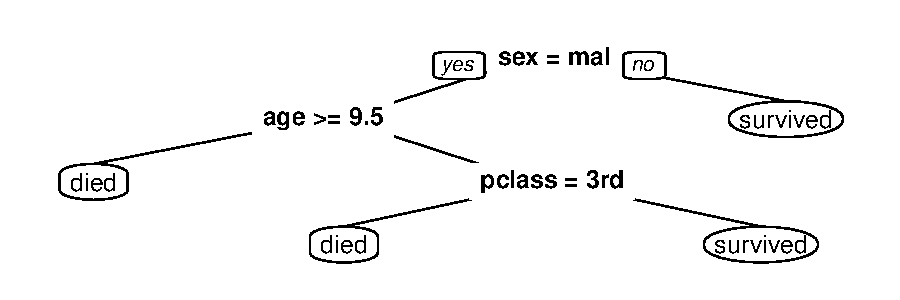
\includegraphics[width=\linewidth]{figure/beamer-titanic-fourth-1} 

}



\end{knitrout}
\end{frame}

\begin{frame}
\frametitle{Ende}

\includegraphics[scale=0.7]{funny/correlation.png}
\end{frame}

\end{document}
